% Created 2012-10-15 Mon 14:56
\documentclass[serif,11pt]{beamer}
\usepackage[utf8]{inputenc}
\usepackage[T1]{fontenc}
\usepackage{fixltx2e}
\usepackage{graphicx}
\usepackage{longtable}
\usepackage{float}
\usepackage{wrapfig}
\usepackage{soul}
\usepackage{textcomp}
\usepackage{marvosym}
\usepackage{wasysym}
\usepackage{latexsym}
\usepackage{amssymb}
\usepackage{hyperref}
\tolerance=1000
\usepackage{fourier}
\providecommand{\alert}[1]{\textbf{#1}}

\title{Quiver in summary}
\author{David Alexander \and Patrick Marks}
\date{\today}
\hypersetup{
  pdfkeywords={},
  pdfsubject={},
  pdfcreator={Emacs Org-mode version 7.8.11}}

\begin{document}

\maketitle


\section{High-level view}
\label{sec-1}
\begin{frame}
\frametitle{What is Quiver?}
\label{sec-1-1}

\begin{itemize}
\item A multiple-read consensus calling algorithm for PacBio reads
\item Takes multiple reads of a given DNA template, outputs best guess
     of template's identity
\item QV-aware conditional random field model to model our sequencing
     errors; a greedy algorithm to find the maximum likelihood
     template.
\item \textbf{Can achieve accuracy >Q50 (i.e. >99.999\%) in applications to de      novo assembly and resequencing using pure PacBio long reads.}
\end{itemize}
\end{frame}
\begin{frame}
\frametitle{How Quiver works}
\label{sec-1-2}

   Quiver uses a greedy algorithm to maximize the likelihood
   $\Pr(\mathbf{R} \mid T)$ in the unknown template $T$.

\begin{itemize}
\item $\Pr(\mathbf{R} \mid T)$ encodes our sequencing error model and is
     specific to a chemistry and enzyme---currently requires a training
     step, which is performed in-house at PacBio.
\end{itemize}

   $\mathrm{QuiverConsensus}$ for reference window $W$: (\emph{Rough sketch})
\begin{itemize}
\item Use reference alignment to identify reads $\mathbf{R}=\{R_1, R_2, \ldots R_K\}$
     corresponding to $W$
\item \emph{Throw away reference---not used in computing consensus}
\item $\hat{T_1} \leftarrow \mathrm{PoaConsensus}(\mathbf{R})$
\item Repeat until convergence:
     $$\hat{T}_{s+1} \leftarrow \hat{T_{s}} +
     \big\{\text{single base mutations } \mu \, \mid
     \Pr(\mathbf{R} \mid \hat{T_s} + \mu) \geq \Pr(\mathbf{R} \mid \hat{T_s}) \big\}$$
\end{itemize}
\end{frame}
\begin{frame}
\frametitle{Where to get Quiver}
\label{sec-1-3}

\begin{itemize}
\item Quiver will be integrated in the 1.4 SMRTanalysis release
\item Until then, you can install it from GitHub, using instructions
     here: \href{http://git.io/AERlEA}{http://git.io/AERlEA}
\item Quiver is open source, under the BSD license, so feel free to
     integrate it in your programs and workflows.
\end{itemize}
\end{frame}
\section{The mechanics, in more detail}
\label{sec-2}
\begin{frame}
\frametitle{Overview of PacBio data}
\label{sec-2-1}

   \begin{figure}
   \centering
     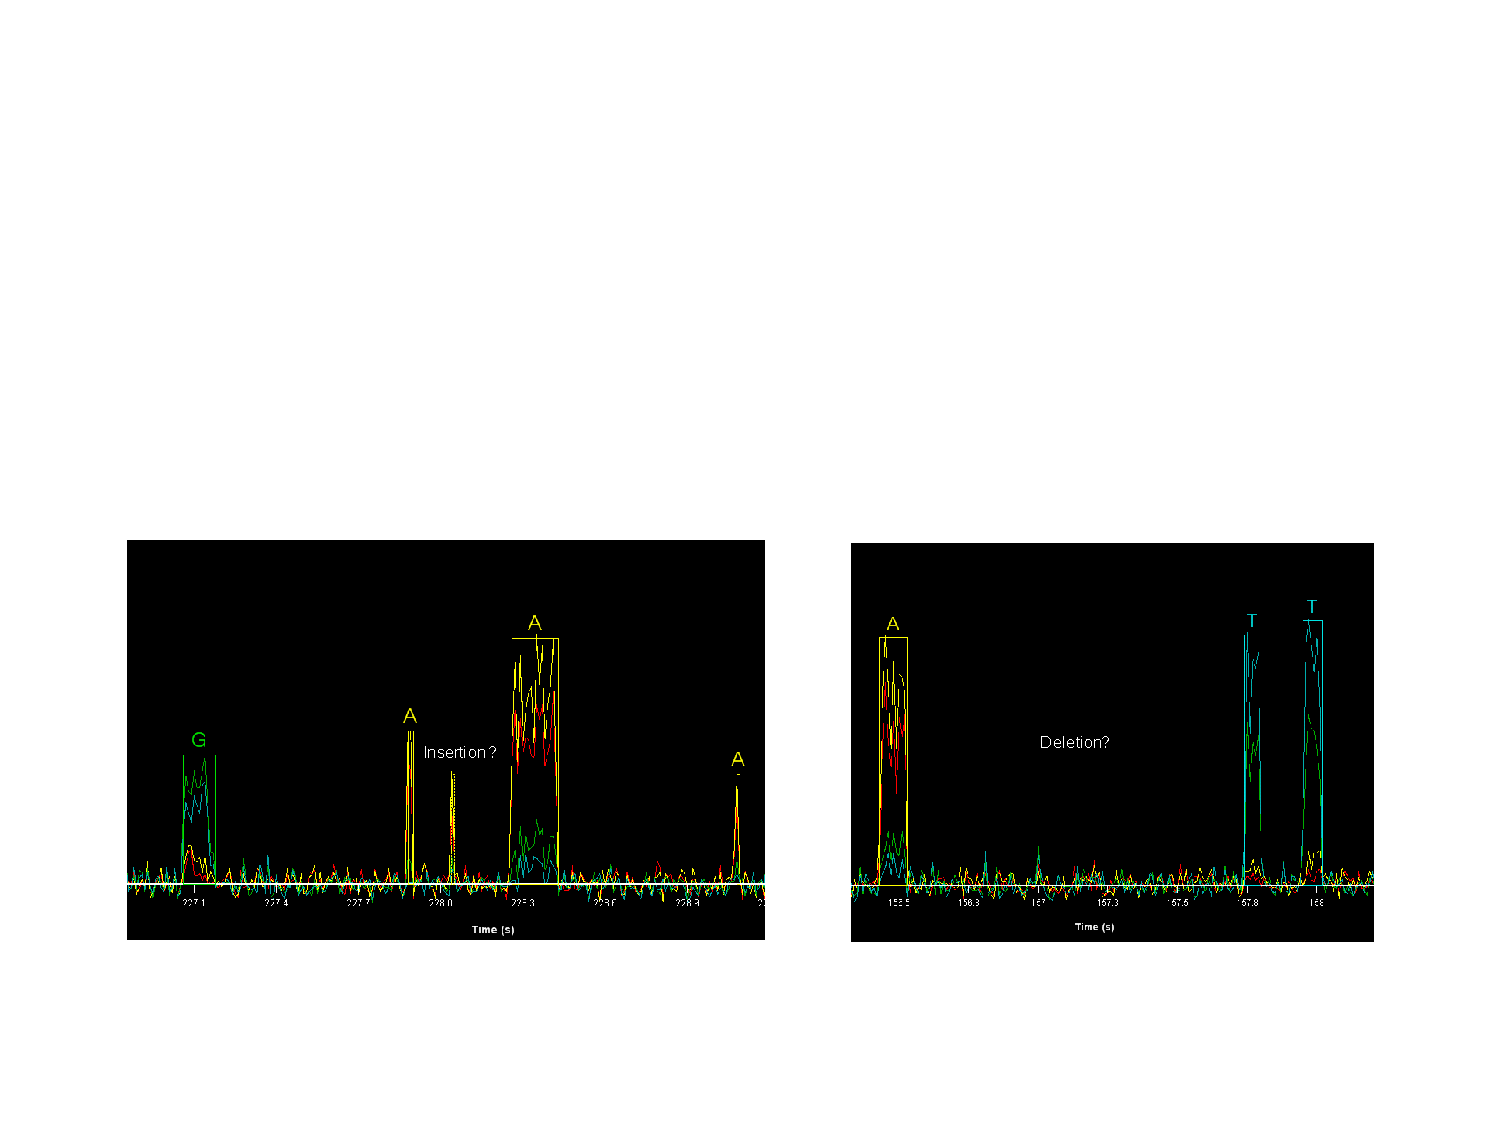
\includegraphics[width=3.5in]{img/traces}
   \end{figure}

\begin{itemize}
\item Very long reads
\item Errors are dominated by indels, not substitutions
\begin{itemize}
\item Mostly cognate extras (homopolymer expansion)
\item Some pulse merging (homopolymer contraction)
\item Some noncognate extras
\item Essentially no substitutions
\end{itemize}
\end{itemize}
\end{frame}
\begin{frame}
\frametitle{Pulse metrics}
\label{sec-2-2}

   In addition to basecalls, the basecaller software includes metrics
   reflecting its confidence against the various types of errors.


\begin{center}
\begin{tabular}{lrrrlr}
 Base  &  Insertion  &  Substitution  &  Deletion  &  Deletion  &  Merge  \\
       &         QV  &            QV  &        QV  &  Tag       &     QV  \\
\hline
 A     &          8  &            12  &        16  &  N         &     14  \\
 T     &          2  &            12  &         5  &  T         &    100  \\
 T     &         11  &            30  &         4  &  G         &     25  \\
 G     &         12  &            30  &        11  &  A         &     11  \\
 G     &          3  &            30  &        16  &  N         &     27  \\
 C     &          6  &            30  &        16  &  N         &     19  \\
 C     &          3  &            19  &         3  &  C         &     21  \\
 G     &          2  &            21  &         4  &  G         &     22  \\
\end{tabular}
\end{center}



   $$QV = -10 \log_{10} p_{error}$$
\end{frame}
\begin{frame}
\frametitle{Definition of pulse metrics}
\label{sec-2-3}


\begin{itemize}
\item \textbf{InsertionQV}, \textbf{SubstitutionQV}: Probability that this base call
     is actually an insertion (substitution) relative to the true
     template.
\item \textbf{DeletionQV}: Probability that the basecaller omitted a base
     relative to the true template, \emph{prior} to this basecall.  Maximum
     likelihood missed base is encoded in \textbf{DeletionTag}.
\item \textbf{MergeQV}: Probability that the basecaller merged together two
     identical adjacent template bases into this basecall.
\end{itemize}

   \emph{All probabilites are phred-encoded.}
\end{frame}
\begin{frame}
\frametitle{How to compute $\Pr(\mathbf{R} \mid T)$?}
\label{sec-2-4}


\begin{enumerate}
\item Reads are assumed independent, so
      $$\Pr(\mathbf{R} \mid T) = \prod_{k=1}^{K}\Pr(R_k \mid T)$$
\item For PacBio, indels are the rule, not the exception, so the model
      considers the possible \emph{alignments}---the ways $T$ can be
      construed to have generated $R_k$:

      $$\Pr(R_k \mid T) = \sum_\mathcal{A} \Pr(R_k \mid T, \mathcal{A}) \mathop{\pi}(\mathcal{A} \mid T)$$

      \emph{This summation can be computed efficiently using a standard Sum-Product dynamic programming approach.}
\end{enumerate}
\end{frame}
\begin{frame}
\frametitle{Sketch of dynamic programming}
\label{sec-2-5}

\begin{itemize}
\item Sum-Product definition:
     \begin{align*}
     A_{ij} \doteq&
     \text{ marginal prob. of an alignment of $R$[0:i+1] to $T$[0:j+1]} \\
     B_{ij} \doteq&
     \text{ marginal prob. of an alignment of $R$[i:I] to $T$[j:J]}
     \end{align*}
\item Sum-Product recursion:
   \begin{align*}
   A_{ij} &= \sum_{m: (i',j') \to (i, j)}   (A_{i'j'} \times \mathrm{moveScore}(m)) \\
   B_{ij} &= \sum_{m: (i, j)  \to (i', j')} (\mathrm{moveScore}(m) \times B_{i'j'})
   \end{align*}
\item For Viterbi approximation, replace \emph{marginal} by \emph{maximum}, replace \emph{sum}
   by \emph{max}.
\end{itemize}
\end{frame}
\begin{frame}
\frametitle{Alignment moves}
\label{sec-2-6}

   \begin{figure}
   \centering
   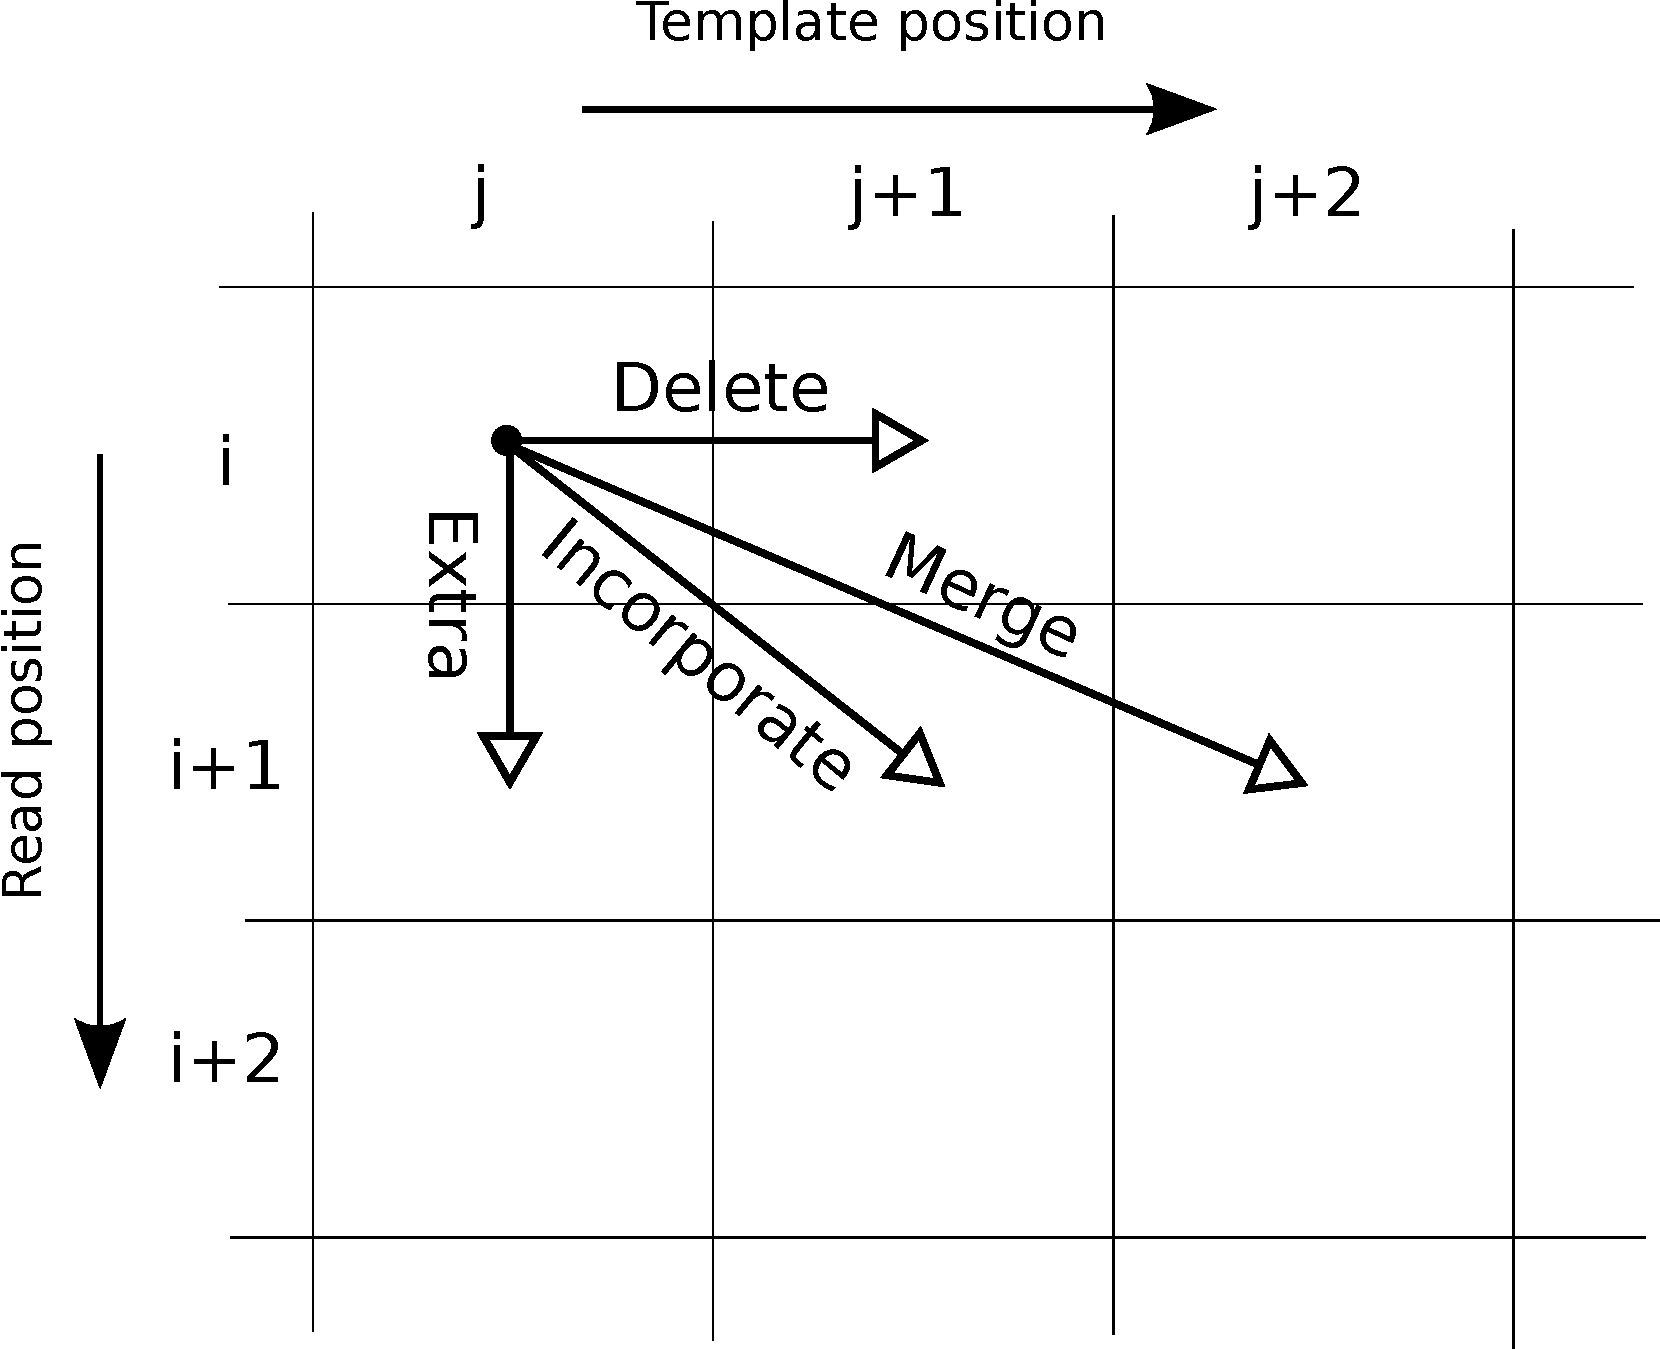
\includegraphics[width=2.5in]{img/moves}
   \end{figure}

\begin{itemize}
\item Additional ``merge'' move helps better account for pulse merging
\end{itemize}
\end{frame}
\begin{frame}
\frametitle{Alignment move scores}
\label{sec-2-7}

\begin{itemize}
\item Modulated by observed pulse metrics (supply more detail here)
\end{itemize}
\end{frame}
\begin{frame}
\frametitle{Efficiently computing $\Pr(R_k \mid T + \mu)$}
\label{sec-2-8}

\begin{itemize}
\item Need to compute score of mutation $\mu$ quickly as this is the
     \emph{rate-limiting operation} in computing the consensus.
\item Do not refill entire $A$, $B$ matrices--we just recalculate two
     columns of $A$ and join with one column of $B$.
\item Exploit identity
     \begin{align*}
     \mathrm{Score}(T) =& A_{IJ} = B_{00} \\
                       =& \max_{m: (i',j') \to (i, j)} A_{i'j'} \times B_{ij},
                       \text{ for \bf{any} $j$}
     \end{align*}
\item Requires $O(L)$ time and space, naively.
\end{itemize}
\end{frame}
\begin{frame}
\frametitle{Banding for memory and CPU efficiency}
\label{sec-2-9}

   \begin{figure}
   \centering
   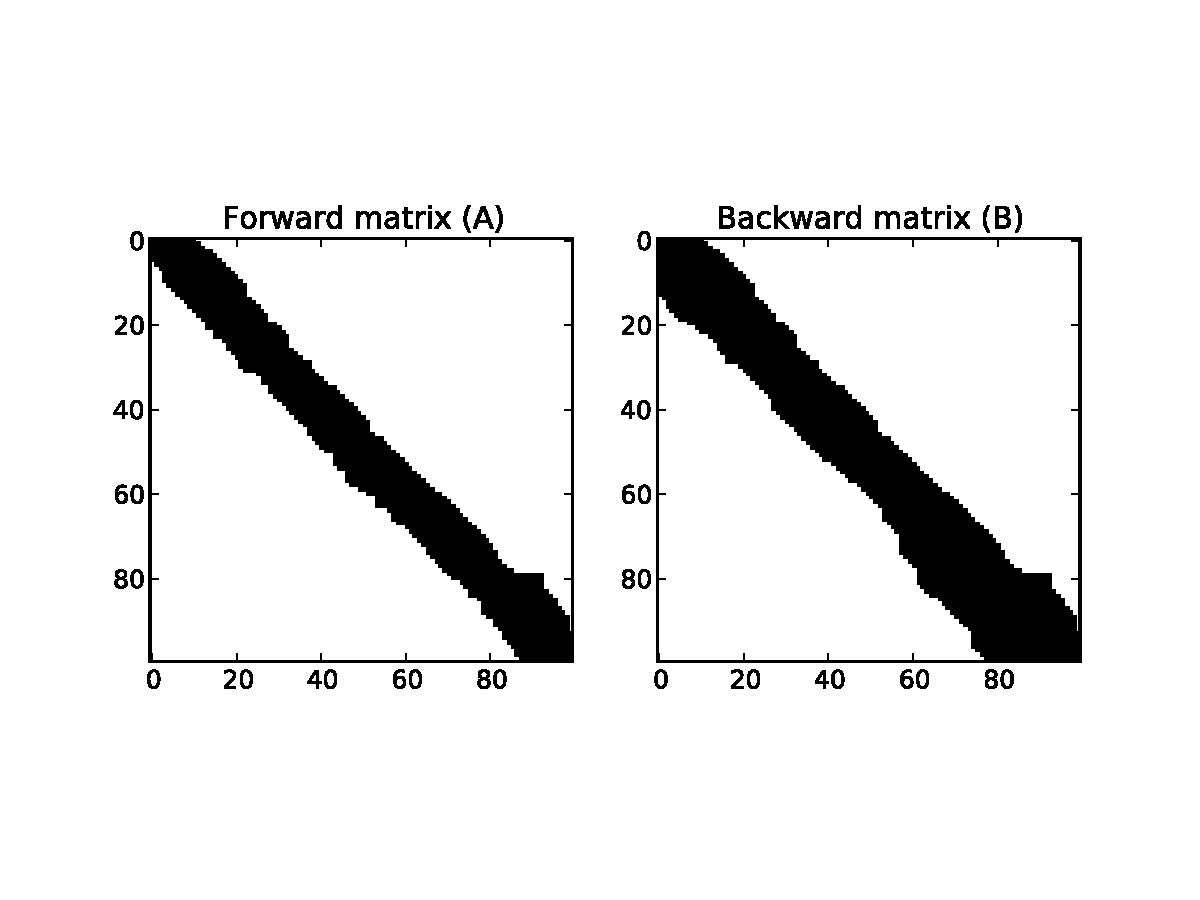
\includegraphics[width=2.5in]{img/sparsity}
   \end{figure}

\begin{itemize}
\item Optimization 1: \emph{banded dynamic programming}: only compute a narrow band of
     high-scoring rows within each column.
\item Optimization 2: Only \emph{store} the bands.

\begin{center}
\begin{tabular}{lll}
                                  &  Naive     &  Banded    \\
\hline
 Initial computation of $A$, $B$  &  $O(L^3)$  &  $O(L^2)$  \\
 Computation of mutation score    &  $O(L)$    &  $O(1)$    \\
 Storage space for $A$, $B$       &  $O(L^2)$  &  $O(L)$    \\
\end{tabular}
\end{center}


\end{itemize}
\end{frame}
\begin{frame}
\frametitle{A good starting point}
\label{sec-2-10}
\begin{columns}
\begin{column}{0.6\textwidth}
%% (ignored)
\label{sec-2-10-1}

\begin{itemize}
\item Prime the ``hill-climbing'' loop with a good starting point
\item We use a heuristic based on Partial-Order Alignment (POA) to for
     a fast approximate consensus.  With 11x coverage it is typically
     >99.5\% accurate.
\item $O(KL^2)$ time; in practice fast enough, but could make faster by
     using a banded approach.
\end{itemize}
\end{column}
\begin{column}{0.4\textwidth}
%% POA Graph Example
\label{sec-2-10-2}

    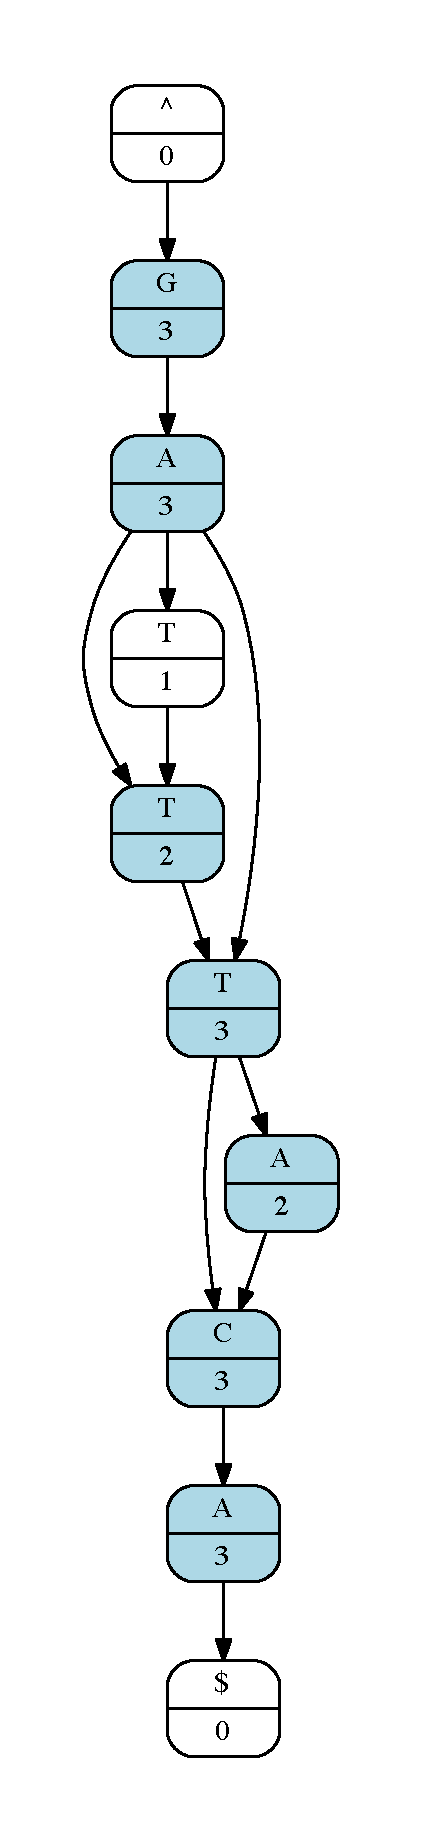
\includegraphics[width=0.45\textwidth]{./img/small-poa.pdf}
\end{column}
\end{columns}
\end{frame}

\end{document}
